\begin{titlepage}
\begin{center}
% Upper part of the page
\textsc{\LARGE An Introduction to}\\[1.5cm]
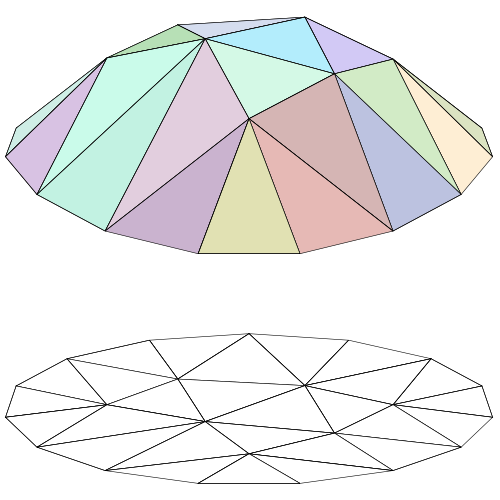
\includegraphics[width=0.5\textwidth]{500px-Piecewise_linear_function2D.png}\\[1cm]    
{ \huge \bfseries \emph{Mathematica} Programming}\\[0.4cm]
\textsc{\Large for Undergraduate Research}\\[0.5cm]
% Title
% Author and supervisor
\begin{minipage}{0.4\textwidth}
\begin{flushleft} \large
\emph{Author:}\\
Robert D. \textsc{French}
\end{flushleft}
\end{minipage}
\begin{minipage}{0.4\textwidth}
\begin{flushright} \large
\emph{Supervisor:} \\
Dr.~Samuel \textsc{Jator}
\end{flushright}
\end{minipage}
\vfill
% Bottom of the page
{\large \today}
\end{center}
\end{titlepage}
